\documentclass{article}

\usepackage{amsmath}
\usepackage{amsthm}
\usepackage{amssymb}
\usepackage{amsbsy}
\usepackage{graphicx}
\usepackage[outdir=./]{epstopdf}
\usepackage[square,numbers,comma]{natbib} 
\usepackage{url}
\usepackage{subcaption}
\usepackage{hyperref}
\usepackage{hyphenat}
\usepackage{pdfpages}
\usepackage{MnSymbol} %udots
\usepackage{afterpage} %\afterpage{\clearpage}
\usepackage{siunitx} %for measurements
\usepackage[figurename=Fig.]{caption}
\usepackage[numbib]{tocbibind} %number references and figure title
\usepackage{authblk}

\setcounter{tocdepth}{2}
\setcounter{secnumdepth}{2}

\let\footruleskip\undefined
\usepackage{fancyhdr}
\pagestyle{plain}

\DeclareMathOperator{\variance}{\mathbb{V}ar}
\DeclareMathOperator{\normal}{N}
\DeclareMathOperator*{\argmax}{argmax}
\DeclareMathOperator{\expectation}{\mathbb{E}}

\newcommand{\addNumber}[1]{\protect\input{#1}\unskip}
\newcommand{\inputNumber}[1]{\protect\input{#1}\unskip}

%to number list of figures
\renewcommand{\listoffigures}{\begingroup
\tocsection
\tocfile{\listfigurename}{lof}
\endgroup}


\title{Detection of defects in additive manufacturing from a single x-ray projection using the empirical null filter}
\date{2019}
\author[1]{S.E.~Lo}
\author[2]{J.W.~Warnett}
\author[2]{G.J.~Gibbons}
\author[2]{M.A.~Williams}
\author[3]{T.E.~Nichols}
\author[1,*]{J.A.~Brettschneider}
\affil[1]{Department of Statistics, University of Warwick, Coventry, CV4 7AL, UK}
\affil[2]{Warwick Manufacturing Group, University of Warwick, Coventry, CV4 7AL, UK}
\affil[3]{Big Data Institute, Old Road Campus, University of Oxford, Oxford, OX3 7LF, UK}
\affil[*]{Corresponding author: julia.brettschneider@warwick.ac.uk, +442476574812}

\DeclareSIUnit\pixel{px}
\DeclareSIUnit\adu{ADU}

\begin{document}\sloppy

\begin{titlepage}
\maketitle

\begin{abstract}
\noindent
\textbf{BACKGROUND}: X-ray computed tomography can be used for defect detection in additive manufacturing (AM). Typically, x-ray projections of an object are taken at a number of angles that are then reconstructed to create a 3D representation of the object inclusive of internal features.
\newline
\textbf{OBJECTIVE}: It was investigated whether it is possible to detect defects based on a single angular projection, avoiding the time-consuming reconstruction process.
\newline
\textbf{METHODS}: An AM sample was manufactured with voids to see if they can be detected. The x-ray projection was compared with a simulation of that projection under the face of uncertainty by treating each pixel as a hypothesis test. To overcome the imperfections of the simulation, the empirical null filter was used to cater for the model misspecification so that sensible inference was achieved.
\newline
\textbf{RESULTS}: Voids with diameters in the order of millimetres were detectable. Simulation studies have shown that statistical properties such as the false discovery rate were preserved.
\newline
\textbf{CONCLUSIONS}: Defect detection in projection space is possible. This work is a contribution towards real-time quality control in AM. The main bottleneck is the multiple evaluations of functions required for robust estimation in the empirical null filter. Speeding up could be possible by implementing the filter on a GPU or exploring further robust estimators.
\newline
\newline
\emph{Keywords:} Additive manufacturing, 3D printing, projection space, hypothesis testing, empirical null, local normalisation, image filtering, voids, defects, quality control
\end{abstract}

\end{titlepage}

\section{Introduction}

Additive manufacturing (AM) is an emerging technology that overcomes many traditional methods such as computer numerical control machining (CNC). In AM, the product is manufactured layer by layer to produce complicated internal and external geometries \citep{ngo2018additive, wong2012review}. One common example of AM technology is fused deposition modelling (FDM) \citep{crump1991fused, crump1992apparatus, stratasys2019what}. A jetting head, or nozzle, deposit the molten material onto a platform or on top of the previous layer. The material is usually plastic in the form of a thin filament. It is heated to just above its melting points, typically \SI{1}{\degreeCelsius} \citep{crump1992apparatus}, so that it cools down within \SI{0.1}{\second} \citep{kruth1991material}. The platform moves, and controlled by a computer, in the $x-y$ axis, or left to right and front to back, to produce a layer. The jetting head can move in the $z$ axis, or up and down, to manufacture the next layer. Powder-based AM such as selective laser sintering \citep{3d2019our, deckard1989method, dtm1990the} can manufacture metal products.

There is a need for product inspection, in particular, quality assessment of the internal structures. The properties of materials produced by AM are not yet fully understood. For example, voids can form between layers which can impact the mechanical properties of the product \citep{ngo2018additive, wang20173d}. In power-based AM technologies, gas can become trapped during the manufacturing process forming gas pores in the manufactured object \citep{tammas2015xct, thijs2010study}. Low wetting ability of the melt pool can cause balling, a phenomenon where spherical or ellipsoidal particles form on the surface of the AM part. They are formed by sintered powder with insufficient contact on the existing layer \citep{gu2009balling, li2012balling}.

Non-destructive testing, such as x-ray computed tomography (XCT), can be used to assess the quality of the product \citep{kruth2011computed, sun2012overview}. The object is held by foam on a turntable and placed between an x-ray source and an x-ray detector. X-ray projections are taken at a series of angles. Typically the x-ray is a cone beam. The x-ray projections are then used to reconstruct the object in 3D \citep{brooks1976principles, feldkamp1984practical, smith1990cone}. 

In AM, XCT is commonly used for the investigation of pores \citep{thompson2016x}. Pores can be classified as defects if the pores are larger than some volume threshold. This threshold controls the probability of the detection of defects \citep{amrhein2014characterization, gandossi2010probability}. The porosity can be estimated by dividing the volume of all of the pores by the volume of solid material in the XCT scan \citep{taud2005porosity}. More accurate methods of measuring the porosity can be done using Archimedes' method \citep{spierings2011comparison}.

An advantage of XCT is that the location of the pores can be visualised. Studies have shown a link between porosity and stress concentration \citep{carlton2016damage, leuders2015fatigue, siddique2015computed}. The location of the pores is a good predictor of fatigue strength \citep{leuders2015fatigue}. In addition to pores, the surface deviation can be measured by aligning the reconstruction with the computer-aided design (CAD) model and measuring any discrepancies \citep{kim2016inspection, lee2015compliance, villarraga2015assessing}.

A disadvantage of XCT is that it involves the acquisition and reconstruction of thousands of projections of the sample. XCT is not an instantaneous process so progress bars are usually featured in XCT marketing such as \emph{Nikon}'s inline quality control \citep{nikon2015inline}. Projection acquisition can take between 15 minutes to a number of hours \citep{warnett2016towards} but more projections would improve the accuracy of the reconstruction \citep{kruth2011computed}.

Instead of reconstructing the object, the analysis can be done on a single x-ray projection itself by comparing it to a simulated projection. It was demonstrated that detection of defects is possible in projection space by comparing two simulated projections with each other, one with defects and the other without \citep{brierley2018optimized}. The simulated projections are made in software called \emph{aRTist} \citep{bellon2012radiographic, bellon2007artist, jaenisch2008artist}. It is however inevitable that information is lost from the jump from reconstruction space to projection space, for example, a CT scan has superior performance in the diagnostic of pneumonia compared to a chest radiograph \citep{hayden2009chest}.

This paper investigates whether defects can be detected from a single x-ray projection. To validate our method, we designed an AM test sample with purposely designed voids to see if they can be detected. The methods section is split into four parts. In Section \ref{subsection:appratus}, a CAD model of the test sample was designed and manufactured using AM. Replicate x-ray projections were obtained of the test sample as well as a simulated projection, without the voids, using \emph{aRTist}. Section \ref{subsection:empiricalnullfilter} explains how the obtained and simulated projections were compared to detect these voids under the face of uncertainty. The uncertainty was modelled using the replicated projections. To overcome the imperfections of the simulation, the empirical null filter was used to cater for the model misspecification so that sensible inference was achieved. The implementation of the empirical null filter is discussed in Section \ref{subsection:computational} and tested on small simulated projections in Section \ref{subsection:simulation}. The results from the simulation and the experiment are shown in the results section. The conclusion section summarises the study along with a discussion on further work.

\section{Methods}

\subsection{Apparatus and Data Collection}
\label{subsection:appratus}

An ABS plastic cuboid (\SI{40}{\milli\metre} $\times$ \SI{40}{\milli\metre} $\times$ \SI{60}{\milli\metre}) with voids was purposefully manufactured to see if they can be detected. The CAD model of the test sample is shown in Fig.~\ref{fig:inference_testObject}. It was manufactured using a \emph{Fortus 400mc (Stratasys, US)} 3D printer. Six voids of each diameter, \SI{2.4}{\milli\metre}, \SI{1.2}{\milli\metre}, \SI{0.6}{\milli\metre} and \SI{0.3}{\milli\metre}, were designed in the CAD model. Voids with diameters \SI{2.4}{\milli\metre} and \SI{0.6}{\milli\metre} were regularly arranged, the other ones were arranged irregularly. The precision of the manufacturing was in the order of $\pm\SI{0.1}{\milli\metre}$ \citep{hanseen2013fortus}.

X-ray projections were obtained using the \emph{Nikon XT H LC 225/320} x-ray CT scanner \emph{(Nikon Metrology, UK)}. The \SI{225}{\kilo\volt} source was used with a $\SI{2000}{\pixel}\times\SI{2000}{\pixel}$ \emph{Perkin Elmer} detector consisting of \SI{200}{\micro\metre} pixels, separated by a distance of \SI{1870}{\milli\metre}. The sample was placed on the manipulator, positioned to obtain a $5.7\times$ magnification resulting in an equivalent pixel size of \SI{35}{\micro\metre}. A voltage of \SI{80}{\kilo\volt} was used with a power of \SI{20}{\watt} resulting in a spot size of \SI{20}{\micro\metre} such that penumbra effects \citep{kueh2016modelling} were negligible. 20 greyscale projections were acquired at an exposure time of \SI{500}{\milli\second}. A shading correction \citep{munzenmayer2003enhancing, young2000shading} was applied to each projection using 20 black (\SI{0}{\kilo\volt}) and 20 white images (\SI{80}{\kilo\volt}) projection to remove intensity influences and variations in pixels of the detector.

19 randomly selected projections, of the test sample, were held out. The remaining projection was used to compare with a simulated projection, obtained using \emph{aRTist} \citep{bellon2012radiographic, bellon2007artist, jaenisch2008artist}. \emph{aRTist} can simulate projections of the sample given the specifications of the CT apparatus, such as the x-ray source and the x-ray detector, and the
CAD of the sample \citep{bellon2011simulation, deresch2012simulating}. \emph{aRTist} was used to obtain a simulation projection as if the voids were not there. Numerical methods were used to align the simulated projection to the obtained projection. The same shading correction was applied to the simulated projection, but instead using a flat black image and a simulated white image.

\subsection{The Empirical Null Filter}
\label{subsection:empiricalnullfilter}

We propose a statistical method to compare a single projection with a simulation of that projection to look for any significant differences which may indicate a defect. It is built on two-tailed multiple hypotheses testing \citep{fisher1970statistical, neyman1933on, pearson1900on} controlling the false discovery rate \citep{benjamini2010discovering, benjamini1995controlling}, conducting an individual test for each pixel. A disagreement too big, relative to the anticipated variance of the projection, will classify that pixel as a positive result. Beforehand, the empirical null \citep{efron2004large} is used to locally normalise \citep{sage2018local, sage2003teaching} the test statistics. This is necessary because the simulation of the projection did not perfectly reproduce the obtained projection, leading to incorrect inference.

Fig.~\ref{fig:flowchart} shows a flowchart which summarises the process of the experiment and defect detection. The CAD model was used as a blueprint for the manufacture of the test sample. Projections of the test sample and the simulated projection were obtained and compared under the face of uncertainty. The uncertainty was modelled using the replicated projections. The test statistics from the comparison were filtered using the empirical null filter and converted to $p$-values. A threshold was used for the $p$-values to classify pixels as positive for defects or not.

For each position $(x,y)$, a test statistic was calculated
\begin{equation}
  Z_{x,y} = 
  \dfrac{
    \text{projection}_{x,y} - \emph{aRTist}_{x,y}
  }
  {
    \sqrt{\widehat{\variance}\left[\text{projection}_{x,y}\right]}
  }
\end{equation}
where $\widehat{\variance}\left[\text{projection}_{x,y}\right]$ is the estimated grey value variance of pixel $(x,y)$ in the projection. The variance model $\widehat{\variance}\left[\text{projection}_{x,y}\right]$ has a linear relationship between the variance and the grey value \citep{yang2010noise}. A gamma distributed generalised linear model \citep{mccullagh1984generalized, nelder1972generalized} was used with an identity link. The fitting of the model was done using the held out replicated projections of the sample (see Section \ref{subsection:appratus}). These replicated projections were manually segmented so that only pixels which represent the test sample were used. This provided variance-mean data, where each pixel is a data point, which was used to fit the variance model. The variance was predicted using the grey value in the simulated projection as the predictor variable.

It was assumed that the grey values were Normally distributed, therefore the test statistics should be approximately Normal as well. Let the test statistic of the pixel at position $(x,y)$ be
\begin{equation}
Z_{x,y}\sim\normal(\mu_{x,y},\widehat{\sigma}_{0,x,y}^2)
\end{equation}
for $x=1,2,\cdots,W$ and $y=1,2,\cdots,H$. $\mu_{0,x,y}$ and $\sigma_{0,x,y}$ are the null mean and null standard deviation at position $(x,y)$. Their estimates, $\widehat{\mu}_{0,x,y}$ and $\widehat{\sigma}_{0,x,y}$ respectively, are called the empirical null mean and empirical null standard deviation. Define the null hypotheses
\begin{equation}
  H_{0,x,y}:\mu_{x,y}=\widehat{\mu}_{0,x,y}
\end{equation}
and the alternative hypotheses
\begin{equation}
  H_{1,x,y}:\mu_{x,y}\neq\widehat{\mu}_{0,x,y} \ .
\end{equation}
The empirical null filter aims to obtain the estimators $\widehat{\mu}
_{0,x,y}$ and $\widehat{\sigma}_{0,x,y}$ for all $x$ and $y$. This is based on the empirical null \citep{efron2004large} where hypothesis testing is done by comparing a test statistic with the empirical distribution of the majority of the test statistics rather than a specified null distribution.

To obtain the estimates, a circular kernel $C_r(x,y)$ with radius $r$ was centred at $(x,y)$. All the pixels captured by the circular kernel and the region of interest (ROI) were pooled together to obtain a kernel density estimate \citep{friedman2001elements, parzen1962on}
\begin{equation}
\widehat{p}_{Z_{x,y}}(z) = 
\frac{1}{nh}
  \sum_{i,j\in K_{x,y}}\phi\left(
    \dfrac{z_{i,j}-z}{h}
  \right)
\end{equation}
where $K_{x,y} = C_r(x,y) \cap \text{ROI}$, $n$ is the number of pixels captured by $K_{x,y}$, $\phi(z)$ is the standard Normal density function and $h$ is the bandwidth. The bandwidth was chosen such that
\begin{equation}
  h = (0.9n^{-1/5}\ + 0.16) \times \text{min}\left(s_{x,y},\text{IQR}_{x,y}/1.34\right)
  \label{eq:inference_ourruleofthumb}
\end{equation}
where $s_{x,y}$ and $\text{IQR}_{x,y}$ are the sample standard deviation and sample interquartile range of the test statistics in $K_{x,y}$, similar to Silverman's rule of thumb \citep{sheather2004density, silverman1986density}. The estimates were obtained by solving
\begin{equation}
\widehat\mu_{0,x,y} = \argmax\widehat{p}_{Z_{x,y}}(z)
\end{equation}
using the Newton-Raphson method and
\begin{equation}
  \widehat{\sigma}_{0,x,y} = \left[
    \left.
      -\dfrac{\partial^2}{\partial z^2}\ln\widehat{p}_{Z_{x,y}}(z)
    \right|_{z=\widehat{\mu}_{0,x,y}}
  \right]^{-1/2}
\end{equation}
\citep{efron2004large}. The test statistics were normalised using
\begin{equation}
  T_{x,y} = 
  \dfrac{
    Z_{x,y}-\widehat{\mu}_{0,x,y}
  }
  {
    \widehat{\sigma}_{0,x,y}
  }
\end{equation}
and converted to $p$-values
\begin{equation}
  p_{x,y} = 2(1-\Phi(|t_{x,y}|)) \ .
\end{equation}

Pixels are classified as positive for defects if its $p$-value is less than some threshold $\alpha$. It controls the per comparison error rate (PCER) \citep{benjamini1995controlling} which is the average proportion of false positives out of all tests or
\begin{equation}
\text{PCER}=\dfrac{1}{N}\expectation\left[\text{number of false positives}\right]
\end{equation}
where $N$ is the number of pixels to test. A typical choice is $\alpha=0.05$ \citep{wasserstein2019moving}. This method of thresholding is flawed because of the possibility of obtaining at least one false positive increases as the number of tests increases \citep{shaffer1995multiple}. For example, suppose none of the pixels represents a defect, then on average, 5\% of these pixels are tested positive and falsely so. This is troublesome and costly because false positives suggest a defect in areas where there are not any defects.

The false discovery rate (FDR) is the average proportion of positives which are false or
\begin{equation}
\text{FDR}=\expectation\left[\dfrac{\text{number of false positives}}{\text{number of positives}}\right]
\end{equation}
where the ratio is defined to be zero when the number of positives is zero. The Benjamini-Hochberg (BH) \citep{benjamini1995controlling} procedure was used to select the threshold such that the FDR is less than 5\%. This allows control for false positives relative to the number of positives. The BH procedure is done by ordering the $p$-values such that $p_{(1)}\leqslant p_{(2)}\leqslant \cdots \leqslant p_{(N)}$ and then using the threshold
\begin{equation}
  \alpha = \frac{0.05 k}{N}
\end{equation}
where
\begin{equation}
  k\text{ is the largest }i\text{ for which }p_{(i)}\leqslant\frac{i}{N}\alpha
  \ .
\end{equation}

\subsection{Computational Implementation}
\label{subsection:computational}

The empirical null filter was implemented using \emph{ImageJ} \citep{abramoff2004image, perez2013image, schindelin2012fiji, schneider2012nih} by modifying the existing class \texttt{RankFilters}. The class contains implementations of filters, such as the mean filter and the median filter, using a circular kernel and multiple threads. Each thread filters a row in parallel.

Line filtering was done from left to right. At the start on the far left, an initial value of the median of all the test statistics in the kernel was used. For the following pixel to the right, the empirical null mean of the neighbouring left pixel was used as the initial point. This was chosen as it was assumed the empirical null mean would vary slowly and smoothly spatially.

When filtering a pixel, the Newton-Raphson method was used to solve for $\widehat{\mu}_{0,x,y}=z$
\begin{equation}
  \dfrac{\partial}{\partial z}\ln\widehat{p}_{Z_{x,y}}(z) = 0
\end{equation}
by using the iterative procedure
\begin{equation}
  z^{(r+1)} =
  z^{(r)}
  -\dfrac{
    \left.
      \dfrac{
        \partial
      }
      {
        \partial z
      }
      \ln\widehat{p}_{Z_{x,y}}(z)
    \right|_{z = z^{(r)}}
  }
  {
    \left.
      \dfrac{
        \partial^2
      }
      {
        \partial z^2
      }
      \ln\widehat{p}_{Z_{x,y}}(z)
    \right|_{z = z^{(r)}}
  } 
\end{equation}
where $z^{(0)}$ is the initial value. A convergence criteria was met when either 10 update steps were taken or when
\begin{equation}
  \log\left[\left|
    \left.
    \dfrac{
      \partial
    }
    {
      \partial z
    }
  \ln\widehat{p}_{x,y}(z)
  \right|_{z=z^{(r)}}
  \right|\right]
  <-5
\end{equation}
at the current step. This was chosen arbitrary to speed up the algorithm without losing too much accuracy. The solution is valid if
\begin{equation}
  \left.
    \dfrac{
      \partial^2
    }
    {
      \partial z^2
    }
    \ln\widehat{p}_{Z_{x,y}}(z)
  \right|_{z=\widehat{\mu}_{0,x,y}}
  < 0 \ .
\end{equation}
Further initial values were generated by sampling from $\normal(z^{(0)}, s_{x,y}^2)$. This was done multiple times until 3 valid solutions were obtained. The best solution, the one with the largest $\ln\widehat{p}_{Z_{x,y}}\left(\widehat{\mu}_{0,x,y}\right)$ out of all the different initial values, was used as the final answer.

To satisfy the condition that the empirical null mean is slowly and smoothly varying, the x-ray projection of the test sample was manually segmented further as shown in Fig.~\ref{fig:inference_segmentFurther}. It was segmented using the edges of the projection of the sample. The empirical null filter was then used on each segment, or ROI, independently, ignoring any pixels outside the ROI the filter was working on. The resulting filtered segments were stitched together to form the resulting filtered image prior to any hypothesis testing.

\subsection{Simulation of Defect Detection}
\label{subsection:simulation}

We tested if the empirical null filter can detect simulated defects from a $\SI{256}{\pixel}\times \SI{256}{\pixel}$ contaminated image. Statistically speaking, a defect is a pixel which has a value not distributed under the null distribution, but instead a alternative distribution. For example suppose $Z_{x,y}|H_{0,x,y}\sim\normal(0,1)$, then a defect would have a value distributed as $Z_{x,y}|H_{1,x,y}\sim\normal(\mu_{1},1)$ where $\mu_1\neq0$. A $\SI{30}{\pixel}\times \SI{30}{\pixel}$ square defect was simulated. A kernel can capture the entire defect if its radius is large enough.

Contamination was simulated by a linear transform of the test statistics $Z_{x,y}$. For example in this experiment, the image was multiplied by 2 and a gradient was added. The null and alternative distributions are
\begin{align}
  Z_{x,y}|H_{0,x,y}&\sim\normal(\mu_{0,x,y},2^2)
  \\
  Z_{x,y}|H_{1,x,y}&\sim\normal(\mu_{0,x,y}+2\mu_1,2^2)
\end{align}
respectively where $\mu_{0,x,y}=0.01(x-x_0)+0.01(y-y_0)$ and $(x_0,y_0)$ is the centre of the image. A simulated contaminated defected image was made by sampling $Z_{x,y}|H_{0,x,y}$ in areas with no defects and $Z_{x,y}|H_{1,x,y}$ with defects. An example of a contaminated square defected image is shown in Fig.~\ref{fig:inference_defectSquare2Example}.

The contamination will cause the test statistics to have larger variance and larger values at the two corners where $\mu_{0,x,y}$ is large. This will cause inflation in false positives.

It was suggested that, as a rule of thumb, the proportion of non-null statistics captured by the kernel should not be larger than $0.1$ to satisfy some assumptions made for the empirical null \citep{efron2004large, schwartzman2008empirical}. In this simulated example, it is about $r>\SI{54}{\pixel}$. A kernel too small would treat the defects as null, making them difficult to detect.

The receiver operating characteristic (ROC) curve \citep{cook2007use, friedman2001elements, green1966signal, hanley1982meaning, metz1978basic} is a parametric plot, displaying the true positive rate (sensitivity) against the false positive rate ($1-\text{specificity}$) for varying thresholds. The area under the ROC curve is a commonly used statistic to quantify the performance of the test \citep{friedman2001elements}. Interpretations of the area do exist \citep{hanley1982meaning, metz1978basic} and discussed thoroughly \citep{cook2007use}.

A simulation study was conducted where a simulated contaminated defected image was filtered for various kernel radiuses for $\mu_1=3$. Hypothesis testing was done on the uncontaminated defected image and filtered contaminated defected image. The area under the ROC curve (AUC) and statistical errors were recorded. This was repeated 100 times by simulating another image and repeating the measurement. To form a baseline to compare with, the results of the uncontaminated defected image were all pooled together to obtain the empirical distribution of the AUC and statistical errors without contamination.

\section{Results}

In the simulation study, defect detection was conducted on a filtered contaminated defected image to investigate the statistical properties of the method. The aim of the filter was to remove the contamination so that sensible inference was achieved. The results from the simulation is shown Fig.~\ref{fig:inference_Experiment_DefectRadiusSquare}.

The area under the ROC curve (AUC) increased with kernel radius which highlighted that a filtered image with a suitable radius kernel can perform almost as well as though there was no contamination. The rule of thumb (see Section \ref{subsection:simulation}) suggest a kernel radius of $r>\SI{54}{\pixel}$ which achieved optimal AUC thus justifies the use of the rule of thumb.

It was observed that there is a kernel radius which minimised the type 2 error. A large kernel radius helped preserve false discovery rate (FDR) control after filtering in these examples but a kernel radius too large can lose statistical power. Keeping the FDR consistent before and after filtering is desirable so it is controlled at a specified level after filtering. For large enough kernel radius, the FDR was controlled at and fluctuates around 5\%.

The running times for the empirical null filter increased with kernel radius. Compared to typical filters, say the mean and variance filter, the empirical null filter is a number of magnitudes slower. The main bottleneck is the evaluation of the density estimate, each step in the Newton-Raphson required the evaluation of $\pi r^2$ data points.

The resulting inference from the test sample is shown in Fig.~\ref{fig:inference_subroiAbsFilterDeg120_inference_radius4}. The larger defects were successfully highlighted by the hypothesis test. The empirical null mean changed face to face, resulting in a clear boundary set by the edges. This suggests that the contamination or inaccuracy from \emph{aRTist} was face dependent.

\section{Conclusion}

Voids in the order of millimetres were detectable which shows potential in defect detection in projection space. This work is a contribution towards real-time quality control in AM.

The empirical null filter catered for inaccuracies made by \emph{aRTist}. This demonstrated that the filter can adjust the null hypotheses according to the data to make a sensible inference. In the experiments, it was found that the FDR level is preserved after filtering.

False positives do occur but this is unavoidable because tests were done at the 5\% FDR level. Typically in the experiments, false positives were isolated single pixels and probably occurred due to random chance. Clusters of positive pixels should raise suspicion. One could create a binary image, assigning a Boolean value whether that pixel was tested positive or not. A binary image filter, such as erode followed by a dilate, can be used to remove isolated positive pixels to emphasise the cluster of positive pixels.

For good results, the faces of the test sample were segmented. This was necessary because the empirical null filter assumes that the null parameters varied spatially smoothly and slowly. Manual segmentation was easy to do because a cuboid has 6 faces. However, segmentation of faces cannot be generalised well to AM products with complicated geometry and curved surfaces.

In the experiment, the angle was chosen to distinguish the designed voids. For general AM products, finding a suitable singular projection angle can be difficult. This problem can be tackled by conducting defect detection on a small number of different angular projections independently to pick up defects hidden behind another.

For a filter to take more than a minute is unacceptable when used on the production line when typical filters can take a fraction of a second. There are a few strategies to accelerate the filter. The empirical null filter may be accelerated using GPUs \citep{eklund2013medical, hwu2011gpu, yang2008parallel}, however efforts to implement the filter in \emph{CUDA} and \emph{C++} is fruitless if there may exist a faster method. Instead, accuracy may be sacrificed for speed by only estimating the null parameters for a number of regularly spaced pixels, the remaining pixels then do estimation through interpolation. The problem is that the assumption of a slow varying null parameter is required much more because of the use of interpolation, this may cause bigger problems due to the face to face transition observed in the experiments. It was found that if a bad solution was found for a point, then that solution would spread its bad solution to neighbour pixels due to the interpolation.

The main bottleneck is the evaluation of the density estimate, each step in the Newton-Raphson required the evaluation of each pixel in the kernel. Perhaps there may be faster methods for density estimation such as fitting a smoothing spline on the histogram \citep{efron2004large}, however, that would require tuning the histogram bins as well as the tuning parameters for the spline. On the other hand, there are methods which use the histogram count and it was found that the estimation of the null parameters was insensitive to the histogram binning \citep{schwartzman2008empirical}.

Estimation of the null parameters is essentially robust statistics, estimating the parameters of the null distribution without being affected by non-null statistics. Potential faster methods than the empirical null could exist in literature \citep{hampel1986robust, huber2009robust, jewson2018principles, maronna2006robust, rousseeuw1987robust}. The EM algorithm \citep{bishop2006pattern, dempster1977maximum} could be used to fit a mixture of Gaussians to identify the null distribution and estimate its parameters. However, the power of hypothesis testing and the empirical null comes from the fact that the alternative distribution does not need to be specified.

\section{Appendix}
Code which reproduces this paper can be found on the \emph{GitHub} page \url{https://github.com/shermanip/oxwasp_insideout}.

\section{Acknowledgements}
This work is funded by EPSRC grant numbers EP/K031066/1 (Inside-out: Statistical methods for Computed Tomography validation of complex structures in Additive Layer Manufacturing) and EP/L016710/1 (EPSRC and MRC Centre for Doctoral Training in Next Generation Statistical Science: The Oxford-Warwick Statistics Programme). We would like to thank Wilfred S.~Kendall for his role as principal investigator.

\settocbibname{References}
\bibliographystyle{acm}
\bibliography{../bib}

\setlofname{Figure Captions}
\listoffigures
\clearpage
\section{Figures}

\begin{figure}[h]
  \centering
  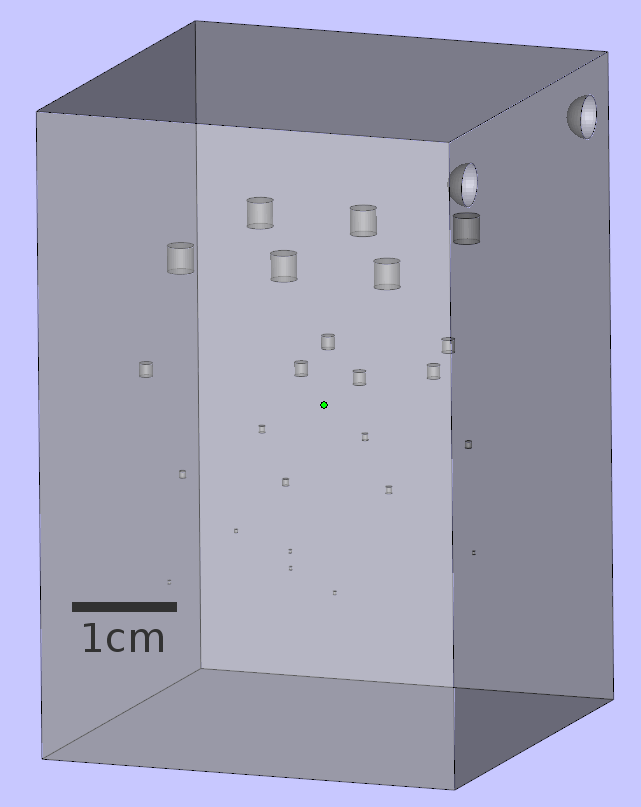
\includegraphics[width=0.49\textwidth]{../figures/inference/TestObject.png}
  \caption{The CAD model of the test sample with voids. Six voids of each diameter, \SI{2.4}{\milli\metre}, \SI{1.2}{\milli\metre}, \SI{0.6}{\milli\metre} and \SI{0.3}{\milli\metre}, were designed in the CAD model. Voids with diameters \SI{2.4}{\milli\metre} and \SI{0.6}{\milli\metre} were regularly arranged, the other ones were arranged irregularly. The scale shown is approximate.}
  \label{fig:inference_testObject}
\end{figure}

\clearpage

\begin{figure}
  \centering
  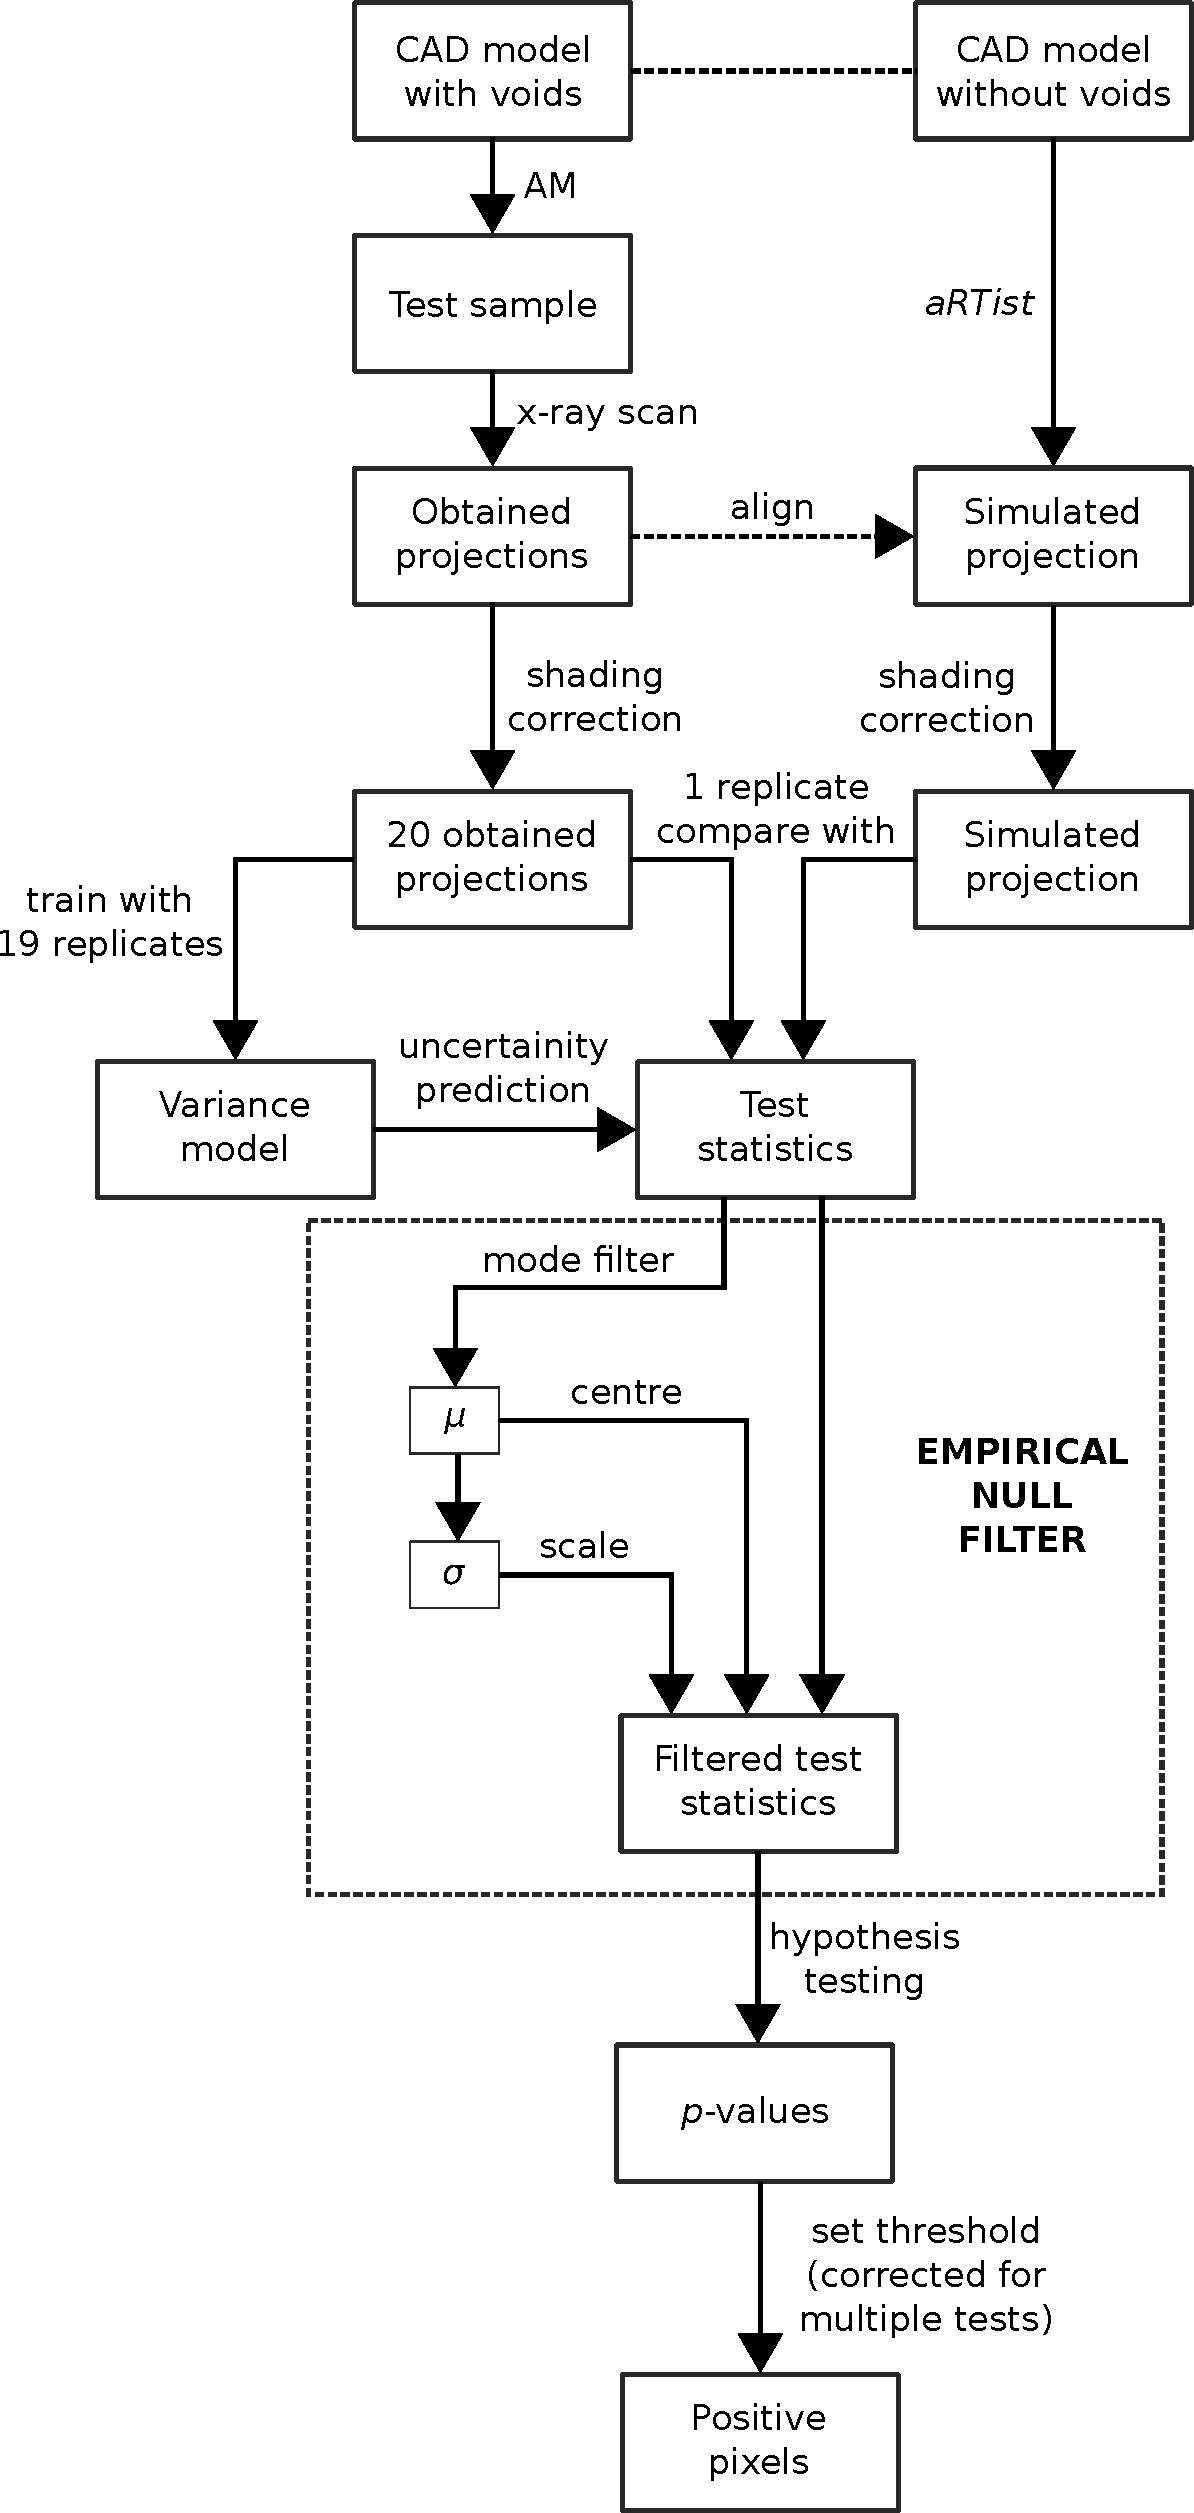
\includegraphics[width=0.7\textwidth]{../figures/flowchart.pdf}
  \caption{Flowchart showing the process of obtaining and comparing a projection of the test sample with the simulated projection.}
  \label{fig:flowchart}
\end{figure}

\begin{figure}
  \centering
  \includegraphics[width=0.49\textwidth]{../figures/inference/DefectExampleSquare40_imageContaminated.eps}
  \caption{A $\SI{256}{\pixel}\times \SI{256}{\pixel}$ contaminated Gaussian image with a $\SI{30}{\pixel} \times \SI{30}{\pixel}$ square defect. The null and alternative distributions are $Z_{x,y}|H_{0,x,y}\sim\normal(\mu_{0,x,y},2^2)$ and $Z_{x,y}|H_{1,x,y}\sim\normal(\mu_{0,x,y}+6,2^2)$ respectively where $\mu_{0,x,y}=0.01(x-x_0)+0.01(y-y_0)$ and $(x_0,y_0)$ is the centre of the image.}
  \label{fig:inference_defectSquare2Example}
\end{figure}

\clearpage

\begin{figure}
  \centering
  \includegraphics[width=0.49\textwidth]{../figures/inference/segment.eps}
  \caption{The $z$ image was segmented further into 7 segments shown by the dotted red lines.}
  \label{fig:inference_segmentFurther}
\end{figure}

\clearpage

\begin{figure}
  \centering
    \centerline{
      \begin{subfigure}{0.49\textwidth}
        \includegraphics[width=\textwidth]{../figures/inference/DefectRadiusSquare_roc.eps}
        \caption{AUC}
      \end{subfigure}
      \begin{subfigure}{0.49\textwidth}
        \includegraphics[width=\textwidth]{../figures/inference/DefectRadiusSquare_type1.eps}
        \caption{Type 1 error}
      \end{subfigure}
    }
    \centerline{
      \begin{subfigure}{0.49\textwidth}
        \includegraphics[width=\textwidth]{../figures/inference/DefectRadiusSquare_type2.eps}
        \caption{Type 2 error}
      \end{subfigure}
      \begin{subfigure}{0.49\textwidth}
        \includegraphics[width=\textwidth]{../figures/inference/DefectRadiusSquare_fdr.eps}
        \caption{FDR}
      \end{subfigure}
    }
  \caption{Area under the ROC curve (AUC) and statistical errors obtained when conducting a hypothesis test on a $\SI{256}{\pixel} \times \SI{256}{\pixel}$ filtered contaminated Gaussian image with a $\SI{30}{\pixel}\times \SI{30}{\pixel}$ square defect for Various kernel radiuses. The dashed lines show the resulting 95\% empirical confidence interval when the hypothesis test was done on the uncontaminated image with a defect. The null and alternative distributions are $Z_{x,y}|H_{0,x,y}\sim\normal(\mu_{0,x,y},2^2)$ and $Z_{x,y}|H_{1,x,y}\sim\normal(\mu_{0,x,y}+6,2^2)$ respectively where $\mu_{0,x,y}=0.01(x-x_0)+0.01(y-y_0)$ and $(x_0,y_0)$ is the centre of the image. The test was conducted at the 5\% FDR level. The box plots summarise the 100 repeated measurements of the simulation.}
  \label{fig:inference_Experiment_DefectRadiusSquare}
\end{figure}

\clearpage

\begin{figure}
  \centering
    \centerline{
      \begin{subfigure}[b]{0.49\textwidth}
        \includegraphics[width=1.05\textwidth, height=4.9cm]{../figures/inference/DefectDetectSubRoiAbsFilterDeg120_radius4_sig.eps}
        \caption{X-ray projection with positive pixels}
      \end{subfigure}
      \begin{subfigure}[b]{0.49\textwidth}
        \includegraphics[width=\textwidth]{../figures/inference/DefectDetectSubRoiAbsFilterDeg120_radius4_logp.eps}\vspace{-1mm}
        \caption{$-\log p$}
      \end{subfigure}
    }
    \centerline{
      \begin{subfigure}{0.49\textwidth}
        \includegraphics[width=\textwidth]{../figures/inference/DefectDetectSubRoiAbsFilterDeg120_radius4_nullMean.eps}
        \caption{Empirical null mean}
      \end{subfigure}
      \begin{subfigure}{0.49\textwidth}
        \includegraphics[width=\textwidth]{../figures/inference/DefectDetectSubRoiAbsFilterDeg120_radius4_nullStd.eps}
        \caption{Empirical null std}
      \end{subfigure}
    }
  \caption{Resulting inference when using the empirical null filter, on each segment independently, with radius $r=\SI{130}{\pixel}$. a) X-ray projection with highlighted red positive pixels at the 5\% FDR level. b) $p$-values on the log scale. c) and d) Empirical null mean and standard deviation.}
  \label{fig:inference_subroiAbsFilterDeg120_inference_radius4}
\end{figure}

\end{document}
